% Generated from committed aggregates; insert inside the relevant report section.
\subsection{Reliability and implications}

\begin{figure}[htbp]\centering
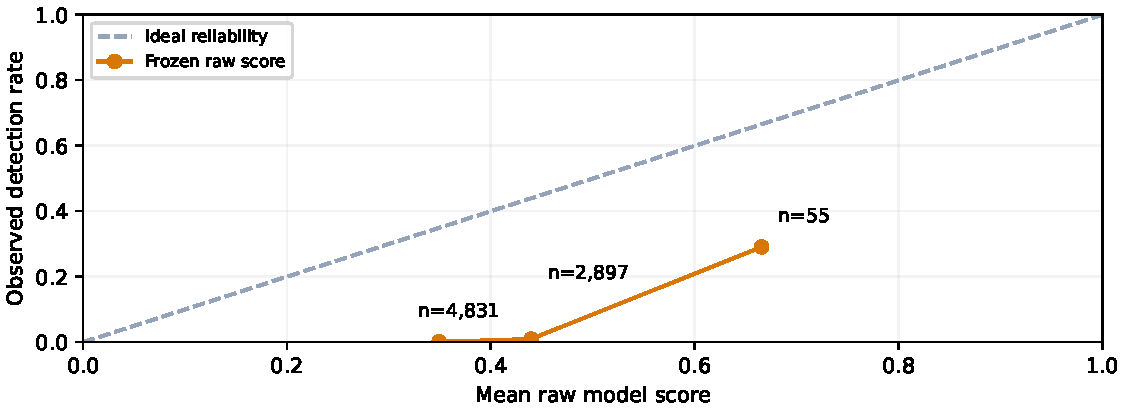
\includegraphics[width=0.94\linewidth]{report/figures/raw_score_reliability.pdf}
\caption{Fixed-bin reliability for the frozen raw score. Bin sizes and observed frequencies do not establish independent-event precision or calibrated percentages.}
\end{figure}

The raw scores overstate observed next-day detection frequencies. The small AP advantage over persistence does not establish practical warning benefit, and Brier/log loss measure overall probability quality rather than calibration alone. We did not fit a correction using final outcomes \cite{mlCalibration,mlFinalEvidence}.

\subsubsection*{Interpretation and recommendations}

The evidence supports a research prototype, not operational dispatch or public risk percentages. False alerts could waste review capacity and erode trust; missed detections could create false reassurance. A future interface should retain human review, label score meaning, provenance and timing, and distinguish satellite non-detection from physical safety. Response capacity and the costs of false versus missed alerts require stakeholder agreement, not invented financial assumptions.

Transfer is limited by sparse early positives, changing prevalence, one supplied season, dependent cells/events, imperfect detection coverage and coarse spatial aggregation. Retrospective publication latency was not simulated. The related Australian multi-source study motivates environmental modelling, but its task, data and headline accuracy are not a like-for-like benchmark for our next-day AP evaluation \cite{mlJois2026}.

Further work needs independent seasons/events, checked observation coverage, suitable fuel information and forecast-time data availability before calibration and response-policy validation. This exposed test must not become a tuning set. The ML contribution completes the auditable comparison; the group must still verify source/licence/map details, domain interpretation, citations, authorship and AI-use records before submission.
